\section{Технологическая часть}
\newsection{Технологическая часть}

\subsection{Выбор языка программирования и среды разработки}
В качестве среды программирования была выбрана операционная система
GNU/Linux. Данная операционная система распространяется по лицензии
GNU GPL и поддерживает стандарт POSIX, поэтому, программное
обеспечение, разрабатываемое для данной операционной системы, будет
переносимо на другие платформы, которые поддерживают POSIX. Также,
одним из преимуществ данной операционной системы является открытость
исходных кодов, что в некоторых случаях позволит более подробно изучить
особенности используемых системных функций. Отлаживать программное
обеспечение в GNU/Linux намного проще, так как нет проблем связанных
политикой безопасности различных антивирусных программ, что присуще
операционной системе Windows.
\newpar
Для реализации программного обеспечения использовался язык C. Данный
язык обладает удобством высокоуровневых языков и возможностями
низкоуровневых языков, что при правильном использовании даст хороший
результат с точки зрения производительности и использования памяти, что в
свою очередь сделает программное обеспечение менее требовательным к
ресурсам и повысит переносимость. Недостатком данного языка является
сложность отладки кода, однако существует различные отладчики, что
упрощает данную проблему.
\newpar
Для создания пользовательского приложения использовался язык Python, версии 3.3,
который более удобен для разработки пользовательского
интерфейса.
\newpar
В число используемых средств также вошли: текстовый редактор vim для
редактирования исходных кодов программы, утилита make для компиляции
исходных кодов и последующей компоновки, отладчик gdb для отладки
программного обеспечения.
\subsection{Описание модулей программного обеспечения}
В данном разделе опишем основные назначения модулей программного
обеспечения. Прототипы и описание пользовательских функций и структур
будут приведены в разделе <<Приложение А>>. Отметим, что алгоритмы работы
этих пользовательских функций описаны в конструкторской части, здесь
же приведена их технологическая составляющая. Используемые типы и
константы приведем в данном разделе. В раздел <<Приложение А>> также
вынесены константы, которые определены в дополнительных файлах.

\subsubsection*{Модуль Network}
Исходные коды данного модуля представлены в файле \textit{network.c}, прототипы
приведены в файле \textit{network.h}. Назначением данного модуля является
установление связи с участниками сети, периодическая посылка
широковещательных сообщения, перехват событий связанных с отправкой и
приемом сообщений. Данный модуль также производит вызов callback-функций
при получении сообщения от сервера или клиента.
\newpar
В данном модуле определены два типа, которые являются указателями на
callback-функции. Данные указатели содержат адреса обработчиков, которые
вызываются, когда необходимо обработать сообщение, пришедшее от клиента
или сервера. Обе функции возвращают целочисленные значения, если оно
равно нулю, то ошибок нет, иначе в зависимости от ненулевого значения
выдается соответствующая ошибка. Ниже приведем определение данных
типов.
\begin{lstlisting}[language=C]
typedef int (*socket_callback)(int sender_sock, const char *received_data, size_t data_len);
typedef int (*server_response_callback)(struct sockets_queue *queue);
\end{lstlisting}
\newpar
Также здесь определены константы, число одновременно прослушиваемых
сокетов, максимальное количество устанавливаемых соединений, и строка
для аутентификации, соответственно.
\begin{lstlisting}
#define SELECT_QUEUE_LEN        5
#define MAX_INTERFACES_COUNT    16
#define IDENT_MSG     "Dzhumagulov_Berezhnoy_IU_7_2013"
\end{lstlisting}

\subsubsection*{Модуль Proto}
Исходный код данного модуля представлен в файле \textit{proto.c}, а прототипы
используемых функций описаны в файле \textit{proto.h}. В данном модуле
описываются правила интерпретации передаваемых сообщений, то есть
протокол, и функции для обработки этих сообщений, а именно функции,
которые преобразуют данные из структуры в последовательность байт или из
последовательности байт получают данные, которыми заполняется структура.
Также имеется дополнительная функция для проверки отдельных бит на
наличие ошибок.
\newpar
Опишем следующие типы:
\begin{lstlisting}
typedef unsigned int pack_id_t; \\ Идентификатор пакета
typedef unsigned int piece_id_t;\\ Идентификатор куска файла
typedef signed int file_id_t;   \\ Идентификатор файла
typedef unsigned short perror_t;\\ Байт для идентификации ошибок
typedef unsigned long long piece_len_t;\\ Длина пересылаемого куска файла
\end{lstlisting}

Соответственно выше определенным типам сопоставляются константы.
\begin{lstlisting}
#define PACK_ID_TSIZE sizeof(pack_id_t)
#define PIECE_NUM_TSIZE sizeof(piece_id_t)
#define FILE_NUM_TSIZE sizeof(file_id_t)
#define PIECE_LEN_TSIZE sizeof(piece_len_t)
#define PROTOCOL_ERROR_TSIZE sizeof(perror_t)
\end{lstlisting}

Ниже представлены номера битов для интерпретации определенных ошибок
протокола.
\begin{lstlisting}
#define PE_FOPEN_FAILURE        0   \\ Ошибка открытия файла
#define PE_FILE_NOT_EXISTS      1   \\ Файл отсутствует на хосте
#define PE_HASH_CMP_FAILURE     2   \\ Неверная хэш-сумма
#define PE_TRNMS_CMPL           3   \\ Передача завершена
#define PE_READ_ACCESS_DENIED   4   \\ Ошибка при попытке прочитать файл
\end{lstlisting}

\subsubsection*{Модуль Cli}
Исходный код и прототипы приведены в \textit{cli.c} и \textit{cli.h} соответственно. В
данном модуле реализован алгоритм работы клиента, а именно алгоритм
реализующий распределение запросов для получения кусков файла, и их
дальнейшую обработку. Ниже приведем используемые константы.
\begin{lstlisting}
#define SRV_UNKN                0   \\ Сервер недоступен
#define SRV_READY               1   \\ Сервер готов к передаче
#define SRV_BUSY                2   \\ Сервер занят


#define TRM_WAITING_SERVERS     0   \\ Ожидание серверов
#define TRM_OBTAINING           1   \\ Получение файла
#define TRM_COMPLETED           2   \\ Передача завершена
#define TRM_UNKN                3   \\ Ошибка при передаче


#define TRME_TOO_MANY_TRM      -1   \\ Слишком много передач
#define TRME_DECODE_ERR        -2   \\ Ошибка при создании сообщения
#define TRME_SOCKET_FAILURE    -3   \\ Возникла ошибка на сокете
#define TRME_NO_ACTIVE_SRVS    -4   \\ Ни один сервер не смог получить запрос
                                    \\ на передачу
#define TRME_ALLOC_FAILURE     -5   \\ Ошибка при выделении памяти
#define TRME_FILE_ERROR        -6   \\ Ошибка при работе с файлом
#define TRME_OUT_OF_MEMORY     -7   \\ Не хватает памяти для всего файла
#define TRME_OPTS_FAILURE      -8   \\ Ошибка при передаче аргуметов
\end{lstlisting}

\subsubsection*{Модуль Srv}
Исходный код приведен в \textit{src.c}, прототипы приведены в \textit{srv.h}. В данном
модуле реализован алгоритм работы сервера. Сервер производит
широковещание через определенный промежуток времен, а при наличии
запрашиваемого файла и соответствующего запроса от клиента начинает
передачу куска файла клиенту. Прототипы функций и структуры приведены
в приложении А.

\subsubsection*{Модуль JSON и MD5}
Данные модули предоставляют стандартные функции для получения хеш-сумм
(модуль MD5) и функций для обмена данными JSON.

\subsubsection*{Модуль Main}
Данный модуль используется для запуска процессов сервера и клиента.
Также содержит функцию, которая позволяет перевести процесс в фоновый
режим работы.

\subsection{Потенциальные ошибки}
В результате работы приложения могут происходить те или иные ошибки,
которые необходимо обрабатывать. Далее рассмотрим основные ошибки и
их обработку.
\begin{enumerate}
    \item Ошибки, возникающие при работе с системными функциями. Данные
        ошибки возникают в результате вызова используемых системных
        функций, например открытие файла, чтение файла или запись в файл, а
        также функция используемые для мультиплексирования ввода\\вывода,
        системные функции, используемые для работы с сокетами и так далее.
        \newpar
        Причиной некорректной работы могут быть, хотя и маловероятно,
        ошибки, возникающие в ходе работы операционной системы,
        неполадки с сетью, или неверные параметры, передаваемые этим
        функциям. В данном случае, если ошибки возникли в результате
        неполадок с ОС, то поведение приложения непредсказуемо, ошибки
        возникающие в результате передачи неверных параметров,
        обрабатываются таким образом, чтобы не нарушалась работа
        приложения, но, если ошибка критическая, то работа приложения
        завершается и выдается сообщение об ошибке. Если ошибки возникают
        из-за неполадок в сети, то работа приложения также завершается.
        \newpar
        Сюда же можно включить ошибки связанные с неполадками в аппаратуре,
        данные ошибки невозможно предусмотреть, поэтому они не
        обрабатываются.
    \item Ошибки, возникающие при завершении работы участников сети.
        Данные ошибки возникают из-за того, что в любой момент времени
        любой из участников сети может завершить работу, в момент передачи
        или приема некоторого файла. Результат обработки таких ошибок
        зависит от количества участников, которые обмениваются файлами.
        \newpar
        Так, если клиент, принимающий файл завершил свою работу, то
        завершают работу все серверы, которые передавали файл этому
        клиенту, если при завершении работы сервера, остаются другие
        работающие сервера, то передача не завершается и не выдается
        сообщение об ошибке, однако когда количество таких серверов равно
        нулю, то клиент завершает работу с ошибкой. В таком случае
        пользовательское приложение выводит сообщение об ошибке.
    \item  Ошибки, возникающие в результате некорректного завершения
        пользовательских функций. Данные ошибки происходят в ситуациях,
        когда пользовательская функция не в состоянии корректно завершить
        свою работу из-за невозможности правильной интерпретации входных
        данных.
        \newpar
        Такие ошибки могут возникать в результате сериализации и
        десериализации сообщений, которыми обмениваются участники, при
        повторном запуске приложения на одном и том же хосте, при
        превышении некоторых ограничений, например при попытке, запустить
        большее количество передач, чем это возможно. При возникновении
        таких ошибок, пользовательские функции возвращают код ошибки,
        которая интерпретируется особым образом. В результате приложение
        выдает сообщение об ошибке или продолжает работу, если ошибка не
        влияет на работу приложения. Например, попытка повторного запуска
        приложения, не влияет на ход работы первого, уже запущенного
        приложения.
\end{enumerate}

\setcounter{figure}{0}
\subsection{Описание графического интерфейса}
Здесь опишем графический интерфейс.
\newpar
При старте пользовательского приложения необходимо ввести логин и
пароль, как это показано ниже на рисунке \ref{login_window}.
\begin{figure}[!hbt]
    \centering
    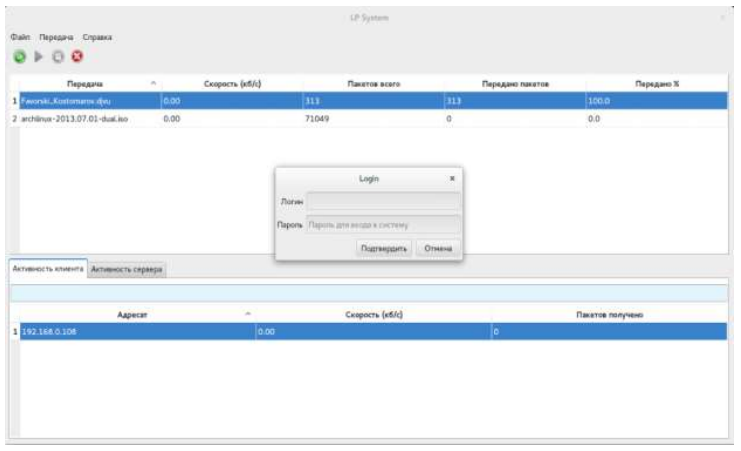
\includegraphics[width=\textwidth]{login}
    \caption{Авторизация}\label{login_window}
\end{figure}
\newpar
В случае ошибки авторизации выводится сообщение, изображенное на рисунке \ref{auth_err}.
\begin{figure}[!hbt]
    \centering
    
\includegraphics{auth_err}
    \caption{Сообщение об ошибке авторизации}\label{auth_err}
\end{figure}
\newpar
После успешной авторизации, становится доступным главное окно. В
главном окне, имеются следующие основные компоненты:
\begin{enumerate}
    \item главное меню --- содержит три вкладки;
    \item окно передач --- окно содержит информацию о текущих передачах;
    \item окно для просмотра активностей с вкладками <<Активность клиента>> и <<Активность сервера>>;
    \item дополнительная панель с кнопками управлениями.
\end{enumerate}

Главное меню приведено на рисунке \ref{main_menu}. При нажатии на вкладки появляются
выпадающее меню. Выпадающее меню <<Файл>> содержит лишь кнопку для
выхода (рисунок \ref{exit_btn}).

\begin{figure}[!hbt]
    \centering
    
\includegraphics{main_menu}
    \caption{Главное меню приложения}\label{main_menu}
\end{figure}
\begin{figure}[!hbt]
    \centering
    
\includegraphics{exit_btn}
    \caption{Выпадающее меню <<Файл>>}\label{exit_btn}
\end{figure}

При нажатии на вкладку <<Передача>>, появляется выпадающее меню, которое
показано на рисунке \ref{transmit}. Для добавления нового торрент файла необходимо
выбрать пункт <<Создать торрент файл>>, при этом появляется окно, куда
необходимо внести информацию о файле, окно представлено на рисунке \ref{add_torrent}.

\begin{figure}[!hbt]
    \centering
    
\includegraphics{transmit}
    \caption{Выпадающее меню <<Передача>>}\label{transmit}
\end{figure}
\begin{figure}[!hbt]
    \centering
    
\includegraphics{add_torrent}
    \caption{Диалог создания нового торрент файла}\label{add_torrent}
\end{figure}

Для добавления торрент файла, который уже существует, необходимо выбрать
соответствующий пункт меню <<Добавить торрент файл>>. При этом
появляется стандартное окно, в котором можно будет выбрать необходимый
файл. Пункт <<Удалить передачу>> удаляет передачу, выделенную в окне
передач. Пункты <<Начать передачу>> и <<Прервать передачу>> позволяют начать
и прервать передачу, соответственно.
\newpar
Ниже приведено выпадающее меню вкладки <<Справка>> (рисунок \ref{help}). Пункт
<<Разработчики>> выводит окно, в котором отображается информация о
разработчиках данного программного обеспечения (рисунок \ref{about}).
\begin{figure}[!hbt]
    \centering
    
\includegraphics{help}
    \caption{Выпадающее меню <<Справка>>}\label{help}
\end{figure}
\begin{figure}[!hbt]
    \centering
    
\includegraphics{about}
    \caption{Окно <<Разработчики>>}\label{about}
\end{figure}

При выборе пункта <<История>> появляется окно журнала, в котором
содержится информация об основных событиях системы, таких как
возникшие ошибки, сообщения о запуске приложения, обнаружение новых
участников и т.д. Пример приведен на рисунке \ref{hist}.

\begin{figure}[!hbt]
    \centering
    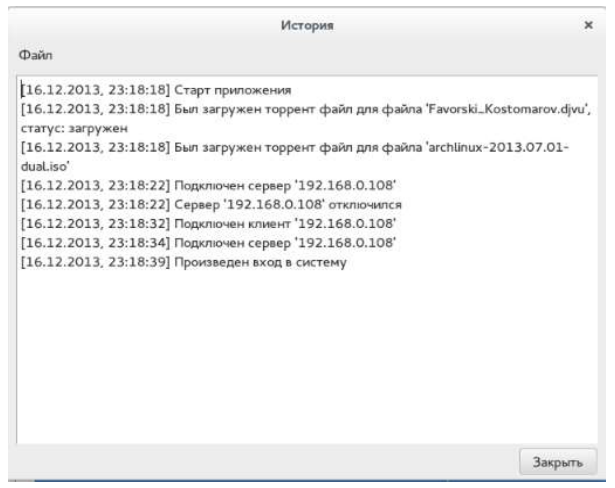
\includegraphics{hist}
    \caption{Окно <<История>>}\label{hist}
\end{figure}

Дополнительная панель с кнопками управления, приведенная на рисунке \ref{buttons},
добавлена для удобства и выполняет те же действия, что и описанные выше
пункты выпадающего меню <<Передача>>, поэтому не будем повторно
описывать их назначение.

\begin{figure}[!hbt]
    \centering
    
\includegraphics{buttons}
    \caption{Панель с кнопками управления}\label{buttons}
\end{figure}

Окно передач содержит сведения о передачах. В данном окне, рисунок \ref{transmitions},
отображается следующая информация:
\begin{enumerate}
    \item скорость передачи (кб/с) -- отображает скорость передачи;
    \item общее количество пакетов -- число пакетов, составляющих некоторую
        передачу;
    \item переданное количество пакетов -- число переданных пакетов на данный
        момент;
    \item процент переданного пакета (\%) -- какая часть передана.
\end{enumerate}

\begin{figure}[!hbt]
    \centering
    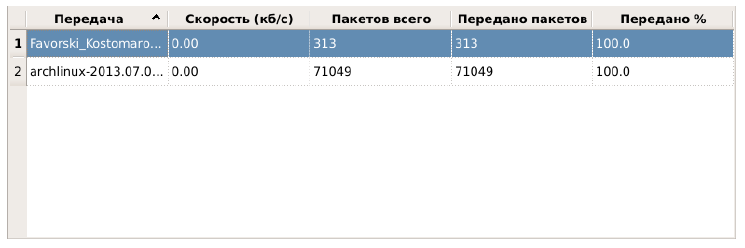
\includegraphics[width=\textwidth]{transmitions}
    \caption{Окно передач}\label{transmitions}
\end{figure}

На рисунке \ref{transmitions} видны две полностью завершенные передачи.
Окно для просмотра активностей с вкладками <<Активность клиента>> на
рисунке \ref{cli_act} и <<Активность сервера>> на рисунке \ref{srv_act} ниже.

\begin{figure}[!hbt]
    \centering
    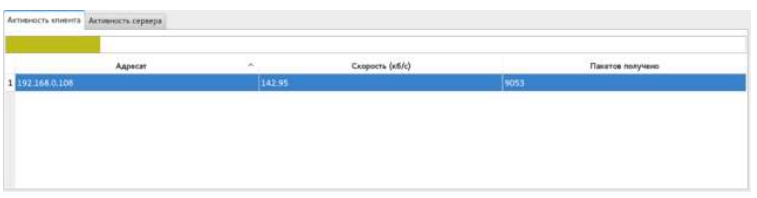
\includegraphics[width=\textwidth]{cli}
    \caption{Вкладка <<Активность клиента>>}\label{cli_act}
\end{figure}

Вкладка <<Активность клиента>> отображает информацию об активности, а
именно:
\begin{enumerate}
    \item адресат -- кто присылает данные;
    \item скорость (кб/с) -- скорость передачи;
    \item пакетов получено – число полученных пакетов.
\end{enumerate}

\begin{figure}[!hbt]
    \centering
    
\includegraphics[width=\textwidth]{srv}
    \caption{Вкладка <<Активность сервера>>}\label{srv_act}
\end{figure}

Вкладка <<Активность сервера>>, отображает информацию о серверах,
которые передают файл, в данной вкладке отображается следующая
информация:
\begin{enumerate}
    \item передача -- к какой передаче относится сервер;
    \item адресат -- кому пересылается;
    \item скорость (кб/с) -- скорость передачи;
    \item передано пакетов -- число переданных пакетов.
\end{enumerate}

\subsection{Тестирование программного обеспечения}
Здесь приведем результаты
 тестирования программного обеспечения. В
 результате тестирования
  необходимо убедиться, что программное
  обеспечение удовлетворяет
   основным требованиям, а также адекватно
   реагирует на внештатные
    ситуации, которые могут возникнуть. Для
    тестирования были использованы три операционные системы Linux Debian,
    которые были запущены на виртуальных машинах VirtualBox.
\subsubsection*{Тестирование работы сети}
Здесь протестируем работу сети, а именно автообнаружение, установление
соединений, а также проверим, чтобы сеть при различных внештатных
ситуациях работала без сбоев.
\newpar
Для того чтобы тестирование было более детальным, вначале, проведем его
без использования графического интерфейса (командная оболочка), а затем
протестируем уже с использованием графического интерфейса.
\newpar
Итак, имеем три ОС со следующими IP-адресами:
\begin{enumerate}
    \item Linux Debian, IP: 192.168.1.3
    \item Linux Debian\_1, IP: 192.168.1.4
    \item Linux Debian\_2, IP: 192.168.1.6
\end{enumerate}

Далее будем писать участник 1, участник 2 и участник 3 подразумевая под
ними Linux Debian, Linux Debian\_1, Linux Debian\_2, соответственно.
\newpar
Протестируем автообнаружение, при этом создадим искусственно
внештатные ситуации, которые заключается в том, что некоторые
участники выходят из сети (по некоторым причинам завершают работу), а
затем снова подсоединяются. Вначале, после того как все трое участников
начали свою работу они должны обнаружить друг друга. Ниже на
рисунках приводятся результаты тестирования и даются комментарии.

\begin{figure}[!hbt]
    \centering
    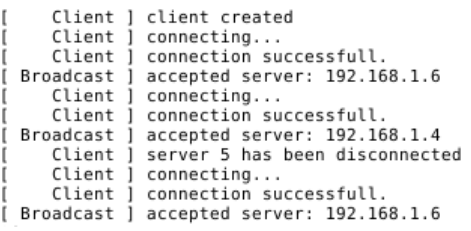
\includegraphics{log_1}
    \caption{Работа участника 1 (процесс-клиент) до прерывания работы}\label{log_1}
\end{figure}
\newpar
На рисунке \ref{log_1} видно, что клиентом обнаружены два участника в сети с IP-адресами
192.168.1.6 и 192.168.1.4, далее следует разрыв соединения с
участником 2 (192.168.1.6) по причине завершения его работы, затем участник 2
снова появляется в сети и снова становится
видимым, далее следует
установление соединения с ним.
\newpar
Допустим, что данный участник 1 по какой-либо причине завершил работу, ниже, на рисунке \ref{log_2} показывается
возобновление его работы. При этом двое других участников снова обнаружены
и, с ними, успешно установлена связь.

\begin{figure}[!hbt]
    \centering
    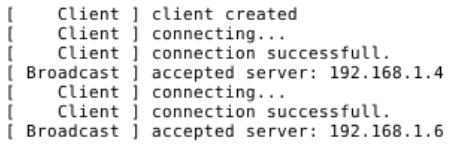
\includegraphics{log_2}
    \caption{Работа участника 1 (процесс-клиент), возобновление работы}\label{log_2}
\end{figure}
\newpar
Сервер в свою очередь производит широковещание, следовательно, его должны
обнаружить остальные участники сети. Ниже, на рисунке \ref{log_3} показано, что два
других участника успешно обнаружили данного участника 1 и установили с
ним соединение. Также на этом же рисунке видно, что с участником 2 потеряна
связь по причине завершения его работы и далее, после возобновления его
работы связь с ним восстанавливается.

\begin{figure}[!hbt]
    \centering
    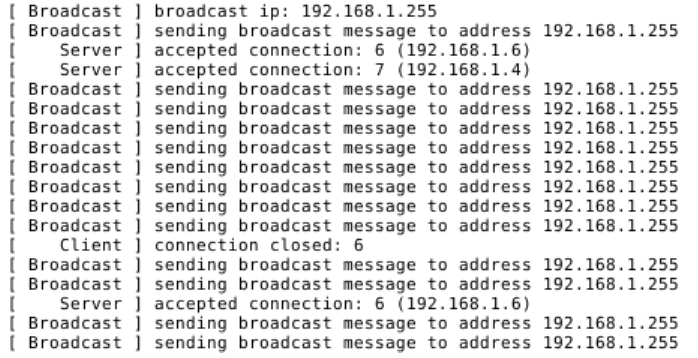
\includegraphics[width=\textwidth]{log_3}
    \caption{Работа участника 1 (процесс-сервер)}\label{log_3}
\end{figure}
\newpar
Рассмотрим работу участника 2 (192.168.1.4). Процесс-клиент участника 2
успешно стартует и успешно устанавливает связь с двумя другими
участниками (рисунок \ref{log_4}). Далее прерывает работу участник 3. После того
как участник 3 возобновил работу соединение устанавливается успешно,
тоже самое можно наблюдать на приведенном выше рисунке \ref{log_1}, с позиции
первого участника.

\begin{figure}[!hbt]
    \centering
    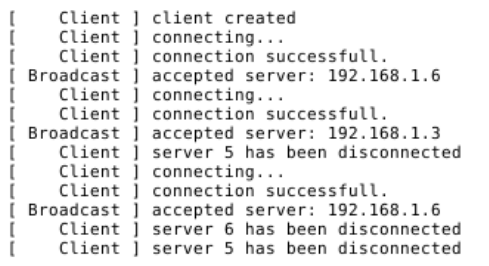
\includegraphics{log_4}
    \caption{Работа участника 2 (процесс-клиент) до прерывания работы}\label{log_4}
\end{figure}
\newpar
Отметим, что данный участник не прерывал своей работы. На рисунке \ref{log_5},
ниже, приведем рисунок с результатами работы процесса-сервера участника 2.

\begin{figure}[!hbt]
    \centering
    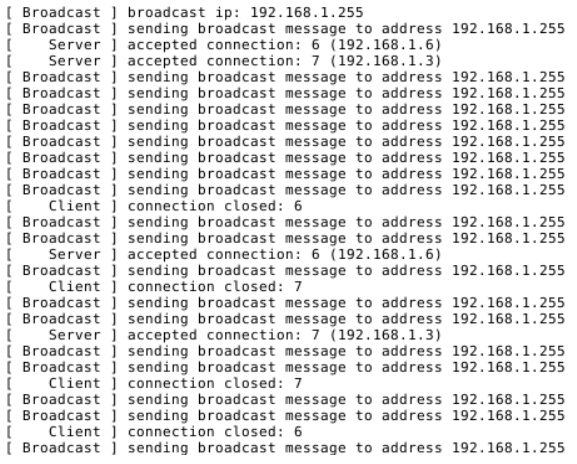
\includegraphics[width=\textwidth]{log_5}
    \caption{Работа участника 2}\label{log_5}
\end{figure}
\newpar
Процесс-сервер успешно запускается и начинает производить
широковещательную рассылку сообщений для того, чтобы другие участники
его обнаружили. Как видно на рисунке \ref{log_5} происходит разрыв связи с двумя
другими участниками, после того как они возобновляют свою работу снова
устанавливается соединение.
\newpar
Рассмотрим работу участника 3. Предположим, что также как и у участника 1
в работе данного участника 3 происходит некоторая ситуация в результате
которой его работа завершается и снова возобновляется. На рисунке \ref{log_6}
приведем пример работы клиента до завершения (прерывания) работы, а на
рисунке \ref{log_7} после возобновления.

\begin{figure}[!hbt]
    \centering
    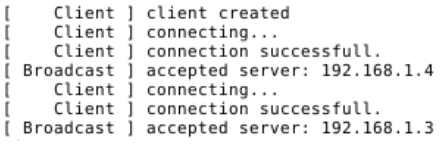
\includegraphics{log_6}
    \caption{Работа участника 3 (процесс-клиент) до прерывания работы}\label{log_6}
\end{figure}
\begin{figure}[!hbt]
    \centering
    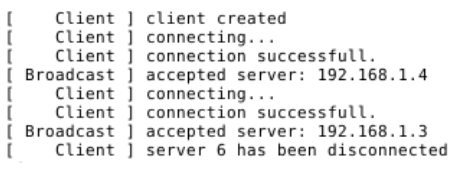
\includegraphics{log_7}
    \caption{Работа участника 3 (процесс-клиент) после возобновления}\label{log_7}
\end{figure}
\newpar
Анализируя приведенные выше результаты работы процесса-клиента
участника 3 видно, что связь устанавливается корректно после запуска и
после возобновления работы участника 3.
\newpar
На рисунке \ref{log_8}, ниже, представлен результат работы процесса-сервера
участника 3.

\begin{figure}[!hbt]
    \centering
    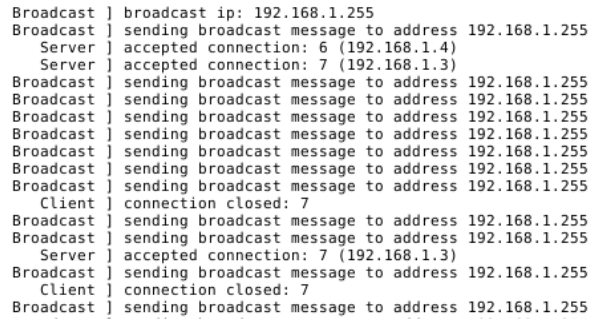
\includegraphics[width=\textwidth]{log_8}
    \caption{Работа участника 3 (процесс-сервер)}\label{log_8}
\end{figure}
\newpar
Как и в предыдущих примерах, видно, что связь устанавливается корректно.
Участники также корректно отображаются в пользовательском приложении,
ниже на рисунках \ref{log_10}, \ref{log_11} и \ref{log_12} приведем примеры панелей «Активность
клиента» для участника 1, участника 2 и участника 3 соответственно.

\begin{figure}[!hbt]
    \centering
    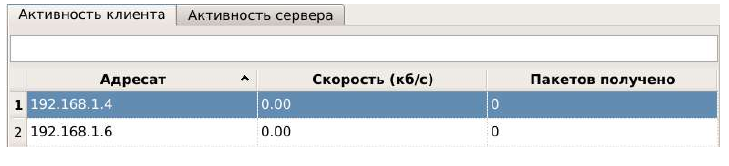
\includegraphics[width=\textwidth]{log_10}
    \caption{Панель <<Активность клиента>> участника 1}\label{log_10}
\end{figure}
\begin{figure}[!hbt]
    \centering
    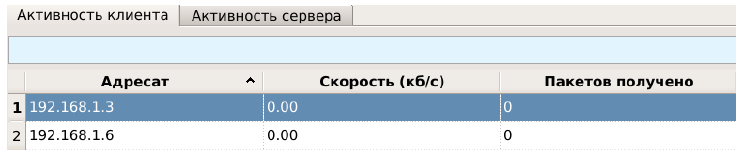
\includegraphics[width=\textwidth]{log_11}
    \caption{Панель <<Активность клиента>> участника 2}\label{log_11}
\end{figure}
\begin{figure}[!hbt]
    \centering
    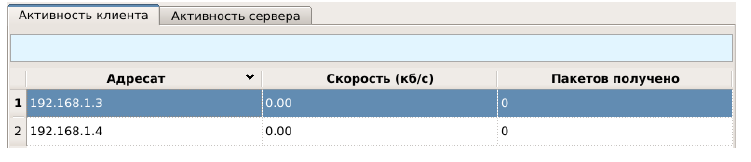
\includegraphics[width=\textwidth]{log_12}
    \caption{Панель <<Активность клиента>> участника 3}\label{log_12}
\end{figure}
\newpar
Было проведено тестирование, из которого можно сделать следующие
выводы:
\begin{enumerate}
    \item обнаружение и установления соединения между участниками
        устанавливается автоматически;
    \item при завершении по каким-либо причинам работы одного из участников,
        работа сети не нарушается, а также это не влияет на работоспособность
        других участников;
    \item при возобновлении работы участников обнаружение и установление
        соединения происходят автоматически;
\end{enumerate}

\subsubsection*{Тестирование запуска демонов}
Процесс-клиент и процесс-сервер являются демонами и должны запускаться
в единственном экземпляре. Попробуем запустить более чем один процесс.
Далее, на рисунке \ref{log_9} показана попытка запуска более чем одного процесса-
клиента и процесса-сервера. Используя команду \texttt{ps –ajx}, которая отображает
демонов, увидим, что были запущены только по одному экземпляру
процессов демонов (рисунок \ref{log_13}). На рисунке \ref{log_14} приведем иллюстрацию
регистрации попытки запуска более чем одного процесса демона.

\begin{figure}[!hbt]
    \centering
    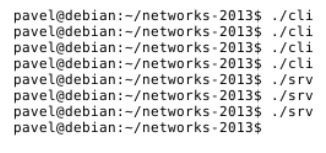
\includegraphics{log_9}
    \caption{Тестирование процесса-демона}\label{log_9}
\end{figure}
\begin{figure}[!hbt]
    \centering
    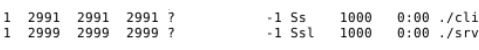
\includegraphics{log_13}
    \caption{Результат команды \texttt{ps -ajx}}\label{log_13}
\end{figure}
\begin{figure}[!hbt]
    \centering
    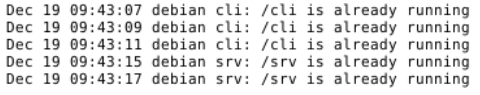
\includegraphics{log_14}
    \caption{Регистрация попытки запуска более чем одного процесса-демона}\label{log_14}
\end{figure}

\subsubsection*{Тестирование передачи файла}
Для тестирования передадим файл \texttt{Favorski\_Kostomarov.djvu} с двух хостов на
третий.
\newpar
Создадим торрент файл, ниже на рисунке \ref{log_15} продемонстрировано создание.
Файл запрашивает участник с IP-адресом 172.20.10.2. У двух других
участников IP адреса 172.20.10.3 и 172.20.10.5, это можно увидеть на том же
рисунке \ref{log_15} во вкладке <<Активность клиента>>. На рисунке \ref{log_16} можно увидеть,
что торрент файл был создан успешно и теперь, данный файл можно
запросить у двух других участников. На рисунке \ref{log_17} можно увидеть, что файл
был передан успешно. Также можно увидеть, сколько пакетов было передано
каждым участником. На рисунках \ref{log_18} и \ref{log_19} можно увидеть вкладку
<<Активность сервера>> двух других участников, при этом отображается имя
переданного файла и число переданных пакетов. На рисунке \ref{log_20} показан
журнал событий, в котором отмечается запуск передачи, на рисунке \ref{log_21} можно
увидеть, что файл был успешно передан, результат заносится в журнал.

\begin{figure}[!hbt]
    \centering
    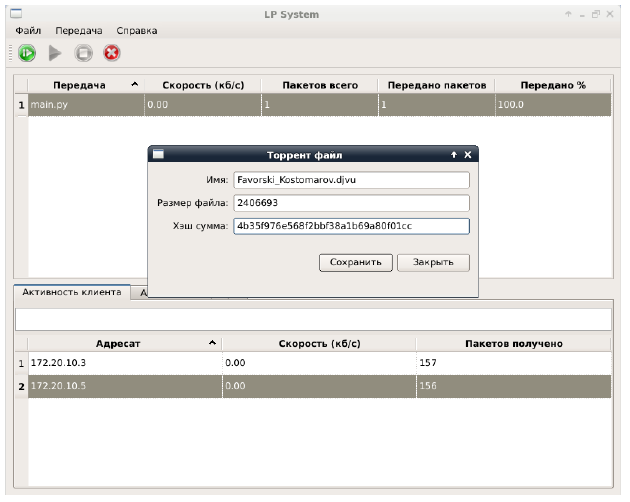
\includegraphics[width=\textwidth]{log_15}
    \caption{Создание торрент-файла}\label{log_15}
\end{figure}
\begin{figure}[!hbt]
    \centering
    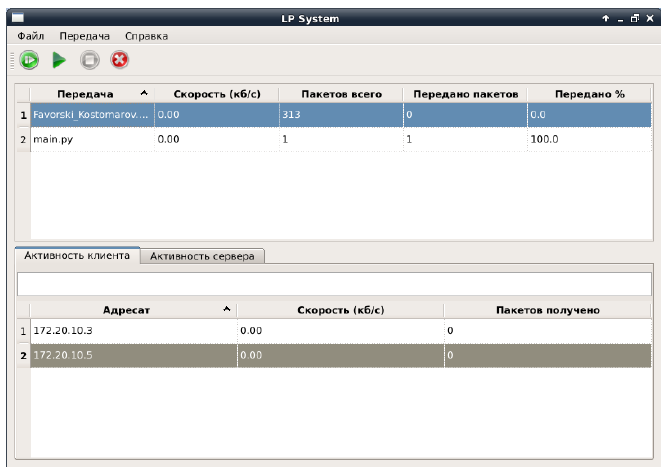
\includegraphics[width=\textwidth]{log_16}
    \caption{Созданный торрент-файл}\label{log_16}
\end{figure}
\begin{figure}[!hbt]
    \centering
    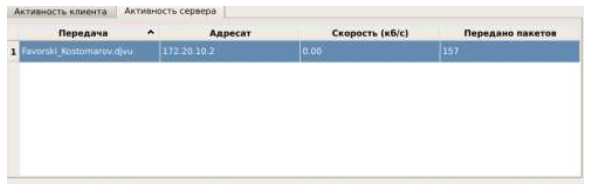
\includegraphics[width=\textwidth]{log_18}
    \caption{Вкладка <<Активность сервера>> участника 1}\label{log_18}
\end{figure}
\begin{figure}[!hbt]
    \centering
    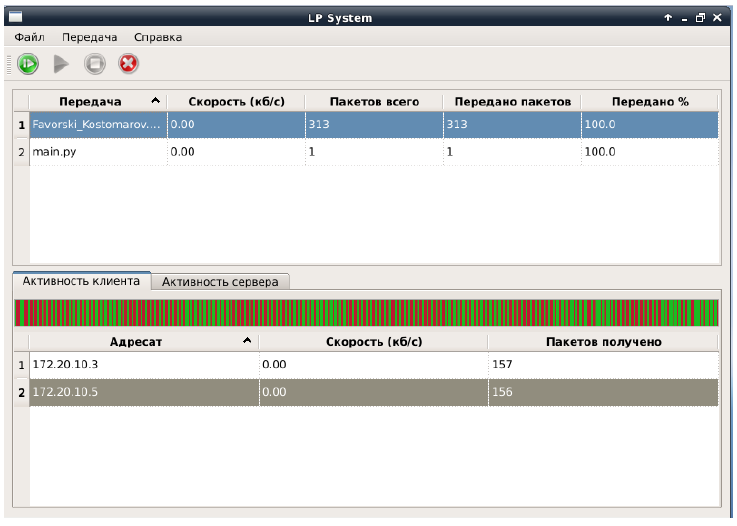
\includegraphics[width=\textwidth]{log_17}
    \caption{Переданный файл}\label{log_17}
\end{figure}
\begin{figure}[!hbt]
    \centering
    
\includegraphics[width=\textwidth]{log_19}
    \caption{Вкладка <<Активность сервера>> участника 2}\label{log_19}
\end{figure}
\begin{figure}[!hbt]
    \centering
    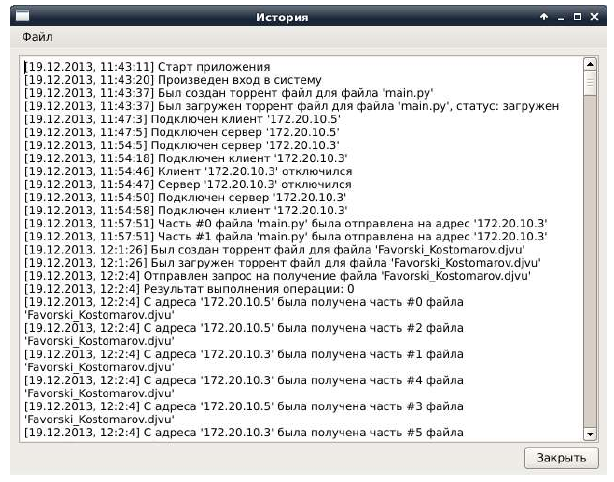
\includegraphics[width=\textwidth]{log_20}
    \caption{Регистрация начала передачи файла}\label{log_20}
\end{figure}
\begin{figure}[!hbt]
    \centering
    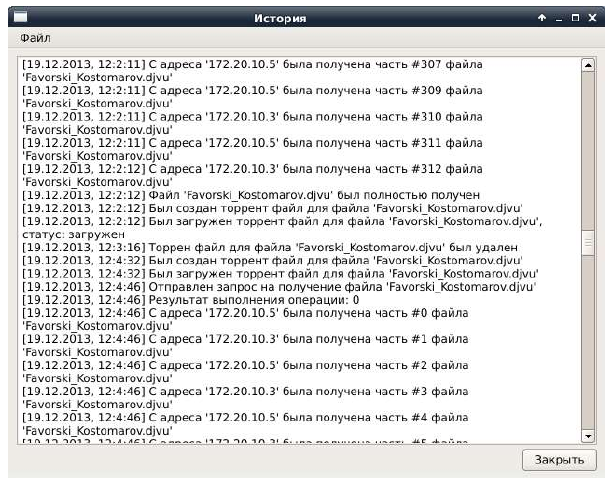
\includegraphics[width=\textwidth]{log_21}
    \caption{Регистрация получения файла}\label{log_21}
\end{figure}

\vfill
\clearpage
\subsection*{Выводы}
\addcontentsline{toc}{subsection}{Выводы}
Был разработан графический интерфейс, который отображает информацию о
передачах и предоставляет пользователю доступ к основным функциям
приложения, а именно:
\begin{enumerate}
    \item создание торрент файлов;
    \item добавление торрент файлов;
    \item запуск, остановка, завершение передач;
\end{enumerate}

Также в приложении имеется журнал, в котором происходит регистрация
основных событий таких как: запуск приложения, возникновение
внештатных ситуаций, добавление нового участника сети, завершение работы
некоторого участника.
\newpar
Приведенные результаты тестирования позволяют сделать вывод о
работоспособности приложения, а также корректную обработку внештатных
ситуаций.

